%!TEX output_directory = .aux
%!TEX copy_output_on_build(true)

\documentclass[11pt,a4paper, titlepage]{article}
\usepackage[a4paper, total={6.5in, 8in}]{geometry}
\usepackage[utf8]{inputenc}
\usepackage{amsfonts}
\usepackage{amssymb}
\usepackage{amsmath}
\usepackage{mathtools}
\usepackage{forest}
\usepackage{subfig}
\usepackage{natbib}
\usetikzlibrary{shapes.geometric,positioning, arrows, trees, positioning, fit, calc}
\usepackage{amsthm}
\usepackage{cleveref}

\title{An Analysis of Smart Voting in Liquid Democracy}
\author{Giannis Tyrovolas}
\date{\today}
\newtheorem{theorem}{Theorem}[section]
\newtheorem{prop}[theorem]{Proposition}
\newtheorem*{remark}{Remark}
\DeclarePairedDelimiter\abs{\lvert}{\rvert}
\DeclarePairedDelimiter\norm{\lVert}{\rVert}


\theoremstyle{definition}
\newtheorem{definition}[theorem]{Definition}
\newtheorem{example}[theorem]{Example}
\newtheorem{corollary}[theorem]{Corollary}
\newtheorem{lemma}[theorem]{Lemma}
\newtheorem{proposition}[theorem]{Proposition}
\newtheorem*{idea}{Idea}

\crefname{definition}{Definition}{Definitions}
\crefname{figure}{Figure}{Figures}
\let\vec\mathbf

% MACROS
\newcommand{\BMM}{\textsc{BoundedMinMax}}
\newcommand{\BMS}{\textsc{BoundedMinSum}}
\newcommand{\BMMS}{\textsc{BoundedMinMaxSum}}
\newcommand{\Maj}{\mathit{Maj}}
\newcommand{\LIQUID}{\mathit{LIQUID}}

\begin{document}

\maketitle

\tableofcontents

\newpage

\section{Context}

Liquid democracy, also referred to as delegative democracy, is a decision-making mechanism that allows greater choice to voters than representative democracy.
Firstly, every voter is allowed to vote directly on an issue. Additionally, delegations are \emph{transitive}. So that a scenario where Alice delegates to Bob and Bob delegates to Charlie is allowed and in this case Charlie votes with the combined power of all three.

One of the first published proposals of this model is Ford's non-technical work in \cite{ford2002delegative}. 
Ford claims that large-scale direct democracy is infeasible and likely undesirable.
It is infeasible because of the frequency of policy decisions and likely undesirable because the ``effective wisdom of the collective can easily turn out to be much worse than its average.''
Representative democracy on the other hand, holds elections every so often. Winners get to represent their constituency while losers gain no representative power.
Additionally, there is a prescribed limit on the total number of elected representatives and every voter can pick from a limited number of representatives.

Delegative democracy is introduced as a balance of the two by challenging the premise that the size of representatives needs to be kept small.
In this model, voters to wish to do so, can vote directly on issues.
Passive voters can delegate to the representatives called delegates.
Delegates are not chosen through time-specific elections but need to canvas voters continually.
When delegates vote they vote with the combined power of all voters that delegate for them.
They can vote on issues directly or they can delegate to other more specialised delegates.
A key-idea is that delegates need not win competitive elections and that delegates have their votes made public for the sake of accountability. 
Ford then introduces notions to replace the parliamentary committees in a setting of liquid democracy.
Then, Ford introduces strengthenings of liquid democracy.
Of interest is the ability to split votes, where agents can delegate fractions of their votes to different delegates. 
Even more interesting is that Ford introduces the ability of agents to submit ``multiple delegation choices in order of preference.'' This is done partly to deal with the case of cycles, where Alice delegates to Bob but also Bob delegates to Alice.
This is one of the key extensions we consider in our work.

An important strand of work in Liquid Democracy is that which considers the ability of Liquid Democracy to find a ground truth. An important contribution is by \citet{kahng2021liquid}. 
The model considers binary issues $\{0, 1\}$ with $0$ being the incorrect outcome and $1$ being the correct outcome. Every voter $i$ has a competence level $0 \leq p_i \leq 1$, which is the probability that a direct vote of voter $i$ is a correct vote.
Further, voters are only able to delegate their votes to a predefined social network. This is claimed to capture the spirit of liquid democracy as voters may be familiar only with some delegates.
These delegates are called the neighbours of $i$.
Further, agents are only allowed to delegate to agents more competent than them by a global constant $\alpha >0$.
So, voter $i$ may delegate to their neighbour $j$ if and only if $p_i + \alpha \leq p_j$. So, $i$ approves of $j$.
This rules out the problem of cyclical delegations a priori as $\alpha >0$

Delegation mechanisms in this context are functions which input an instance of the model and output, for each voter $i$, a delegation probability distribution over the agents $i$ approves of.
After, the delegation mechanism decides the delegation distribution for each voter the majority rule is applied, with ties broken arbitrarily.
The probability that the group votes for the correct outcome for a particular instance of the model $G$ and a delegation mechanism $M$ is $P^M(G)$.
A particular delegation mechanism is that of direct voting denoted as $D$.
An important distinction, the authors make are between \emph{local} and non-local delegation mechanisms. \emph{Local} delegation mechanisms are delegation mechanisms where the resulting distribution for agent $i$ depends only on the set of agents $i$ approves of, the set of neighbours of $i$ and an arbitrary ranking $\pi_i$.
For example, every voter voting directly or voting for a random approved delegate is a local mechanism. Voting for the most competent approved delegate or voting for a delegate with a specific identifier are non-local mechanisms.

In this setting, \citeauthor{kahng2021liquid} compare liquid democracy to direct voting. They set out two desirable properties.
Mechanism $M$ satisfies the \emph{do no harm} property if, the improvement that direct voting $D$ has on $M$ applied to any instance of size $n$ vanishes as $n$ tends to infinity.
Formally, for every $\varepsilon > 0$ there exists $N$ such that for all $n > N$ and graphs $G$ of size $n$, $P^M(G) - P^D(G) \geq - \varepsilon$.
Mechanism $M$ satisfies the \emph{positive gain} property if for some constant $\gamma > 0$ and for every large enough $n$ there exist instances with size $n$ such that $M$ outperforms $D$ by $\gamma$.
Note that in both cases 

After this lengthy setup, we arrive at the key result of the paper. No local delegation satisfies both \emph{positive gain} and \emph{do no harm}.
As this is an impossibility result, the requirement that agents are only able to delegate to more informed voters seems to strenghten this result rather than weaken it.
Something mitigating the impossibility result is that the do no harm property focuses on worst case instances rather than average instances.
It is still undecided if there exist local delegation mechanisms that do no harm \emph{on average}.
The paper's secondary result is that if we bound voters competence away from 0 and 1, a simple non-local delegation mechanism exists.
The mechanism iteratively constructs delegations by having voter $i$ delegate their vote to the most competent approved voter of $i$ that has at most $\sqrt[3]{\log n}$ already delegating to them.

This model was further considered by \citet{caragiannis2019contribution} after the preprint of \citet{kahng2021liquid} was published.
The authors first disagree with the premise that $\alpha$-delgations capture the essence of disagreeing opinions.
They claim that a voter $i$ with competency level of $0.1$ would never delegate to voter $j$ with a competency level of $0.6$ as voter $i$ would consider $j$ to be horribly misinformed.
Instead in their paper, for $\alpha \geq 0$, if $p_i \geq \frac{1}{2}$, agent $i$ would be able to delegate only to agents with $p_j > p_i + \alpha$, and symmetrically if $p_i \leq \frac{1}{2}$.
A small objection to this modelling is that the model implicitly gives meta-information to agents with competency less than $\frac{1}{2} - \varepsilon$ or greater than $\frac{1}{2} + \varepsilon$. Nevertheless, the paper only proves hardness results and so this meta-information strenghtens the results.

A more important objection to $\alpha$-delegations is that there are cases where voting for someone less competent can be beneficial.
A simple example is that for $2k + 1$ voters, let $p_1 = \ldots = p_k = 0$, $p_{k+1} = \ldots = p_{2k} = 1 - \varepsilon$ and $p_{2k+1} = 1 - 2\varepsilon$.
Agents $k+1, \ldots, 2k$ form a star with agent $2k+1$ in the middle.
Then, if agents are restricted to delegating to more competent agents, all voters need to independently vote for $1$ for the majority to vote for 1.
The probability of this occurring is bounded by $(1 - \varepsilon)^k$ which tends to 0 as $k$ goes to infinity.
On the contrary if agents delegate to the central node the probability of correct vote is $1 - 2\varepsilon$.

The paper then proves the following two hardness results.
For any local delegation mechanism $M$ and any $\delta > 0$ there are instances where direct voting or complete dictatorship outperforms $M$ by $\frac{1}{2} - \delta - \alpha$.
Their construction does not use transitive delegations and so apply to simpler models of Liquid Democracy like Proxy Voting.
The more striking hardness result is that even if we consider \emph{non-local} delegation mechanisms the optimal delegation is hard to approximate.
By a reduction to a special version of \textsc{3-SAT} approximating the success rate of the optimal delegation structure within an additive term of $\frac{1}{16}$ is NP-hard.



\newpage
\section{Preliminaries}

\subsection{Ballots}

A single-issue election consists of a finite set of voters that vote on a single issue. 
Each voter is presented with a finite set of alternatives to pick from. 
A special alternative is the \emph{abstention} represented by $*$. 
Finally, there is an aggregation function that decides the result of the election. 
Formally:

\begin{definition}[Single-issue election]
    A \emph{single-issue election} consists of a tuple $\langle N, D, r\rangle $ where $N = \{1,..., n\} $ is a finite non-empty set of voters. The set $D$ is a finite set with $\abs{D} \geq 1$. The function $r \colon D^n \longrightarrow D$ is a resolute aggregation function that inputs the votes of every voter and outputs the outcome of the election.
\end{definition}

Throughout this work we will focus on single issues with a binary set of outcomes. 
That is because all of our hardness results hold for binary issues and we can easily extend them to $n$-ary issues. 
Therefore, unless otherwise stated we will consider $D = \{0, 1\}$.

The model we will consider generalises the above and allows each voter to submit a smart ballot. 
A smart ballot is a preference list of smart votes. 
Each smart vote is a function whose domain is a subset of $N$. 
A special requirement is that the final preference in the preference list is a direct vote on an alternative in $D$. 
Formally:

\begin{definition}[Smart Ballots]
    A \emph{smart ballot} of an agent $a$ is an ordering $( (S^0, F^0) > \ldots > (S^{k-1}, F^{k-1}) > d)$ where $k \geq 0$. Each $S^h$ for $h \leq k$ is a subset of $N$ and $F^h \colon D^{S^h} \longrightarrow D$ is a resolute non-constant aggregation function. We also have that $d \in D$.   
\end{definition}

Further when relevant we will consider $F^{k}$ to be the constant function with output $d$. 
Now, in most cases the sets $S^h$ are implicit and we will drop any mention of them. 
That is supported by the fact that we will treat two functions $F, G$ as identical if they are extensionally equal. 
Additionally we will disallow a voter to delegate to themselves. 
This is formalised by the following definition:

\begin{definition}[Valid Smart Ballot]
    A \emph{valid smart ballot} of an agent $a$ is a smart ballot $B_a$ such that for all $ 0 \leq s < t \leq k$ $F^s$ is not equivalent to $F^t$. Additionally for all $0 \leq t \leq k$, $a \notin S_t$.
\end{definition}


We collect the $n$ smart ballots into a smart profile $\mathbf{B}$.

Throughout this work it will be meaningful to restrict the functions agents can delegate from. The most notable classes of functions we will consider are: 

\begin{itemize}
    \item Direct delegations to voter $v$ denoted by $\mathit{LIQUID} = \{\mathit{id}_v \mid v \in N\}$, where $\mathit{id}_v$ is the identity function applied to the vote of voter $v$.
    \item Boolean functions in conjunctive normal form denoted by $\mathit{BOOL}$. 
    \item Monotone boolean function in conjunctive normal form denoted by $\mathit{MON}$-$\mathit{BOOL}$.
\end{itemize}

\subsection{Unravellings}

Now that we have defined each agent's preferences we need to formalise how to make sense of these preferences. To do so, we use \emph{unravelling procedures} to determine each agent's vote.

\begin{definition}[Unravelling Procedure]
    An \emph{unravelling procedure} is any computable function $\mathcal{U}$ where $\mathbf{B} \mapsto^\mathcal{U} \vec{d}$ with $\vec{d} \in D^n$.
\end{definition}

The reason we need to consider unravelling procedures is that smart ballots can create cycles.
Different choices on how to ``unravel'' cycles will produce different outcomes.
For the majority of this work we will focus on the mathematical and computational properties of different unravelling procedures.


Now as each outcome is calculated it is important for agents to know which preference level was used to compute their vote. 
To do so we introduce the notion of a certificate:

\begin{definition}[Certificate]
    A \emph{certificate} $\mathbf{c} \in \mathbb{N}^n$ for a profile $\mathbf{B}$ is a vector where for each $a \in N$ such that $B_a = (B_a^0 > \ldots > B_a^{k_a})$, the entry $c_a \in [0, k_a]$ corresponds to the preference level for agent $a$.  
\end{definition}


Something that will be of high importance is that functions of interest can be calculated on partial input.  
For example, consider majority rule denote as $\mathit{Maj}$. For a variable $a$, $\mathit{Maj}(1, 1, a)$ will always resolve to 1 regardless of agent $a$'s vote. 
We refer to these cases as \emph{necessary winners} as in Konczak's and Lang's work \cite{konczak2005voting}.
We formalise this in the following definition where we use $\Delta$ to denote placeholder values.

\begin{definition}[Necessary winner extensions]
    Let $F \colon D^n \longrightarrow D $ be a function.
    We define $F' \colon \left\{D \cup \left\{\Delta\right\}\right\}^n \longrightarrow D \cup \left\{\Delta\right\}$ function $F$'s \emph{necessary winner extension}. 
    We set for all $\vec{d} \in D^n$, $F'(\vec{d}) = F(\vec{d})$.
    Now for $\vec{d} \in \left\{D \cup \left\{\Delta\right\}\right\}^n$, let $i_1, i_2, \ldots, i_m$ be the indices such that $d_{i_j} = \Delta$.
    Let $\vec{d}[x_1, \ldots, x_m]$ denote the vector $\vec{d}$ where $x_j$ replaces the value at index $i_j$. Then, if for some $y \in D$ and for all $\vec{x} \in D^m$, $F(\vec{d}[\vec{x}]) = y$ then $F'(\vec{d}) = y$.
    Otherwise $F'(\vec{d}) = \Delta$.
\end{definition}

To actually use our agents' preferences we need to introduce the concept of a consistent certificate. 
Consistent certificates are certificates where the vote of each agent is determined by the votes of other agents using the functions in their smart ballots. Formally:

\begin{definition}[Consistent certificate]
    For a profile $\mathbf{B}$, a certificate $\mathbf{c}$ is \emph{consistent} if there is an ordering $\mathbf{\sigma} \colon N \longrightarrow \{1,\ldots, n\}$ of agents starting from vector $\vec{X}^0 = \{\Delta\}^n$ with placeholder values $\Delta$ for all agents, iteratively constructs an outcome vector of direct votes $\vec{X} \in D^n$ as follows for $\sigma(a) = z \in [1,n]$. For ease of notation we abbreviate agent $a$'s $c_a$th function, $F_a^{c_a}$ to $F$.
    \[
        X^z_a = F'(\vec{X}^{z-1} \restriction_{S^{c_a}_a} ).
    \]
    Here, $X_a$ represents agent $a$'s entry in $\vec{X}$. 
    The restriction of vector $\vec{X}$ in $S$, written as $\vec{X} \restriction_S$, is a vector indexed by $S$ where for each $s \in S$,  $(\vec{X} \restriction_S)_s = X_s$.


\end{definition}


Now, we are only interested in consistent certificates as these are the ones that respect the agents' votes. We will denote the set of consistent certificates of a profile $\mathbf{B}$ as $C(\mathbf{B})$.
It is good that there is only one outcome matched to each consistent certificate regardless of the ordering $\sigma$. The following proposition is proven by Colley et al. \cite{grandi}.

\begin{proposition}
    If a consistent certificate $\mathbf{c}$ can be given by two orderings $\sigma$ and $\sigma'$ of the agents, then the orderings yield the same outcome $X_\mathbf{c} \in D^n$.
\end{proposition}

Consequently, when we refer to consistent certificates are enough to determine every agent's vote. 
Now that we have settled the framework it's time to consider some ``good'' certificates. 
There is a very natural ``cost'' in this scenario and that is using a lot of the later preferences of each agent. 
So, we can set two very natural ways of minimising this cost. 
We can attempt to minimise the sum of the costs or in a more egalitarian spirit attempt to minimise the maximum cost. 
Formally:

\begin{definition}[MinSum]
    For a given profile $\mathbf{B}$, the \textsc{MinSum} unravelling procedure is defined as:
    \[
        \textsc{MinSum}(\mathbf{B}) = 
        \left\{X_{\mathbf{c}} \bigm| \mathrm{arg} \min_{\mathbf{c} \in C(\mathbf{B})} \sum_{i=1}^n c_i\right\}.
    \]
\end{definition}

\begin{definition}[MinMax]
    For a given profile $\mathbf{B}$, the \textsc{MinMax} unravelling procedure is defined as:
    \[
        \textsc{MinMax}(\mathbf{B}) = \left\{X_{\mathbf{c}} \bigm| \mathrm{arg} \min_{\mathbf{c} \in C(\mathbf{B})} \max (\mathbf{c}) \right\}.
    \]
\end{definition}

The above unravelling procedures have already been introduced and studied by Colley et al. \cite{grandi}. 
A natural extension of \textsc{MinMax}, not studied is that of \textsc{MinMaxSum} that selects from the \textsc{MinMax} certificates the ones with minimum sum. 
Formally:

\begin{definition}[MinMaxSum]
    For a given profile $\mathbf{B}$, the \textsc{MinMaxSum} unravelling procedure s defined as:
    \[
        \textsc{MinMaxSum}(\mathbf{B}) =  \left\{ X_{\mathbf{c}}\mid \arg  \min_{\vec{c} \in \mathit{minC}(\mathbf{B})} \sum_{i=1}^n c_i \right\}.
    \]
    where $\mathit{minC}(\vec{B})$ is the set of consistent certificates that minimise the maximum $c_i$. 
\end{definition}


\newpage



\section{Complexity Results}

\subsection{Hardness Results}

In order to study the computational properties of the unravelling procedures we set them up as decision problems.

\begin{definition}[\textsc{BoundedMinSum}]
    Let \textsc{BoundedMinSum}$_\mathcal{F}$ be the decision problem with input a target constant $M$ and a smart profile $\mathbf{B}$ which uses functions in the class $\mathcal{F}$. 
    The YES instances are those with a consistent certificate  $\vec{c}$ with $\sum_i c_i \leq M$. 
\end{definition}

\begin{definition}[\textsc{BoundedMinMax}]
    Let \textsc{BoundedMinMax}$_\mathcal{F}$ be the decision problem with input a target constant $M$ and a smart profile $\mathbf{B}$ which uses functions in the class $\mathcal{F}$. The YES instances are those with a consistent certificate  $\vec{c}$ with $\max(\vec{c}) \leq M$. 
\end{definition}

\begin{definition}[\textsc{BoundedMinMaxSum}]
    Let \textsc{BoundedMinMaxSum}$_\mathcal{F}$ be the decision problem with input target constants $M, S$ and a smart profile $\mathbf{B}$ which uses functions in the class $\mathcal{F}$. The YES instances are those with a consistent certificate  $\vec{c}$ with $\max (\vec{c}) \leq M$ and $\sum_i c_i \leq S$.
\end{definition}


Now, \textsc{BoundedMinSum} and \textsc{BoundedMinMax} have been studied by Colley et al \cite{grandi}.
They proved that \textsc{BoundedMinSum}$_\mathit{LIQUID}$ and \textsc{BoundedMinMax}$_\mathit{LIQUID}$ are poly-time computable and that \textsc{BoundedMinSum}$_\mathit{MON\text{-}BOOL}$ and \textsc{BoundedMinMax}$_\mathit{BOOL}$ are NP-complete.
We improve on these hardness results and conclude some inapproximability results.

Before delving any further we can consider the trivially easy cases. 
For any function class $\mathcal{F}$, \textsc{BoundedMinSum}$_\mathcal{F}$ and \textsc{BoundedMinMax}$_\mathcal{F}$ are trivially solvable if the maximum size of the ballot is 1.

Now, let $\lor$ be the binary logical OR and $\land$ be the binary logical AND. Then:

\begin{proposition}[Hardness of \textsc{BoundedMinSum}]
    Suppose $\mathit{LIQUID} \cup \{\lor, \land\} \subseteq \mathcal{F}$. Then \textsc{BoundedMinSum}$_\mathcal{F}$ is NP-hard, even if the maximum size of a smart ballot is 2.    
\end{proposition}

\begin{proof}
    We reduce from the NP-hard problem of \textsc{3-SAT}.
    Let $\varphi = \bigwedge_{i = 1}^k t_i $ a \textsc{3-SAT} instance on boolean variables $x_1, \ldots, x_n$ with $t_i = l_a \lor l_b \lor l_c $ where $l_a, l_b, l_c$ correspond to literals of variables $x_a, x_b, x_c$ or their negations.
    
    We first define constant voter \underline{zero}, that always votes for 0, so that $B_{\text{\underline{zero}}} = (0)$.

\tikzset{circ/.style={circle,draw, solid, inner sep=0pt,minimum size=10mm}}


For each variable $x_i$ we construct a voter $x_i$ with voting profile $B_{x_i} = (  \text{\underline{zero}} > 1) $. These are drawn in Figure \ref{fig:votes}. We denote the first preferences as solid lines and second preferences as dashed lines.


We then construct gadgets for each term $t_h$. 
These gadgets will have the property that they incur no additional cost if $t_h$ is satisfied and a cost of at least one if $t_h$ is not satisfied. We prove this for the four different structures of a term $t_h$.

\begin{figure}
    \centering
    \subfloat[\underline{zero} voter]{
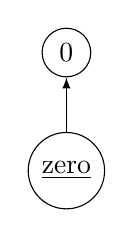
\begin{tikzpicture}[edge from parent/.style={draw,-latex}, align=center,node distance=2cm]

\node[circle,draw] (z){\underline{zero}} [grow = up]
    child{node [circle,draw]{0}
    };
\end{tikzpicture}
    }
    \qquad
    \subfloat[Voter $x_i$]{
        \begin{tikzpicture}[edge from parent/.style={draw,-latex}, align=center,node distance=2cm]

            \node[circ] (x){$x_i$} [grow = up]
            
                child{node[circ] (1){1}  edge from parent [dashed]}
                child{node [circ] (z){\underline{zero}}{
                    child{node[circ](0){0}}}
                };
            \end{tikzpicture}
    }
    \caption{Setting up the variables voters}
    \label{fig:votes}
\end{figure}

\textbf{Case} $x_i \lor x_j \lor x_k$: We construct fresh voters $t_h$, $a$, $b$, and $c$ with smart profiles:

\begin{align*}
    &B_a = (t_h > 0) \\
    &B_b = (x_i \lor a > 0) \\
    &B_c = (x_j \lor b > 0) \\
    &B_{t_h} = (x_k \lor c > 0).
\end{align*}
Now, we analyse when first preferences of the additional voters can be resolved without producing cycles. If $x_i = 1$ then $x_i \lor a = 1$ and $b$ resolves to vote $1$ using the first preference. 
Hence, $b \lor x_j = 1$ and $c$ resolves to $1$ using first preference. 
Similarly, $t_h$ resolves to $1$ and then $a$ resolves to $1$ using only first preferences. 
Similarly, if $x_j = 1$ or $x_k = 1$, agents $c$ and $t_h$ respectively will resolve to $1$ and so all fresh agents will resolve their votes using only first preferences.

Now, suppose $x_i = x_j = x_k = 0$. Suppose there is an ordering $\sigma \colon N \longrightarrow \{1,\ldots, m\}$ that gives rise to a consistent certificate using only the first preferences of agents $a, b, c, t_h$. Then, $\sigma(t_h) < \sigma(a)$ as $a$ needs $t_h$ to be resolved. Further, $\sigma(c) < \sigma(t_h)$ as $x_k = 0$ and so $c$ determines the clause $x_k \lor c$. Similarly, $\sigma(b) < \sigma(c)$ and $\sigma(a) < \sigma(b)$. This leads to the contradiction that $\sigma(a) < \sigma(a)$. Therefore, no such ordering exists and if $x_i = x_j = x_k = 0$, one of the fresh voters $a, b, c, t_h$ will need to incur a cost of at least $1$.

\textbf{Case} $\overline{x_i} \lor x_j \lor x_k$: We construct additional voters $t_h$, $a$, $b$ and $c$, with smart profiles:

\begin{align*}
    &B_a = (t_h > 0) \\
    &B_b = (x_i \land a > 0) \\
    &B_c = (x_j \lor b > 0) \\
    &B_{t_h} = (x_k \lor c > 0).
\end{align*}
This is demonstrated by Figure \ref{fig:MinSum:1nots}.

\tikzset{circ/.style={circle,draw, solid, inner sep=0pt,minimum size=10mm}}
    \begin{figure}
        \centering
    \subfloat[\centering Case $\overline{x_i} \lor x_j \lor x_k$]{{
    \begin{tikzpicture}[edge from parent/.style={draw,-latex}, align=center,node distance=1.75cm]
    
    \node[circ] (xi){$x_i$};
    \node[circ, right of=xi] (a){$a$};
    

    \node[circ, below of=xi] (xj){$x_j$};
    \node[circ, below of=xj] (xk){$x_k$};
    \node[circ, right of=xj] (b){$b$};
    \node[circ, right of=xk] (c){$c$};
    
    
    \node[draw, dashed, rounded rectangle, fit={(xi)(a)}] (elli1) {};
    \node[draw, dashed, rounded rectangle, fit={(b)(xj)}](elli2) {};
    \node[draw, dashed, rounded rectangle, fit={(c)(xk)}](elli3) {};

    \node[circ, below of=elli3](t){$t_h$};
    
    \draw [->] (b) -- (elli1) node[midway,left]{$\land$};
    \draw [->] (c) -- (elli2) node[midway,left]{$\lor$};
    \draw [->] (t) -- (elli3) node[midway,left]{$\lor$};
    \draw [->] (a.east) to [bend left=90] (t.east) {};
    
    \end{tikzpicture}
    \label{fig:MinSum:1nots}
    }}
    \qquad
    \subfloat[Case $\overline{x_i} \lor \overline{x_j} \lor x_k$]{{
        \begin{tikzpicture}[edge from parent/.style={draw,-latex}, align=center,node distance=1.75cm]
    
            \node[circ] (xk){$x_k$};
            \node[circ, right of=xk] (a){$a$};
            
        
            \node[circ, below of=xk] (xj){$x_j$};
            \node[circ, below of=xj] (xi){$x_i$};
            \node[circ, right of=xj] (b){$b$};
            \node[circ, right of=xi] (c){$c$};
            
            
            \node[draw, dashed, rounded rectangle, fit={(xk)(a)}] (elli1) {};
            \node[draw, dashed, rounded rectangle, fit={(b)(xj)}](elli2) {};
            \node[draw, dashed, rounded rectangle, fit={(c)(xi)}](elli3) {};
        
            \node[circ, below of=elli3](t){$t_h$};
            
            \draw [->] (b) -- (elli1) node[midway,left]{$\lor$};
            \draw [->] (c) -- (elli2) node[midway,left]{$\land$};
            \draw [->] (t) -- (elli3) node[midway,left]{$\land$};
            \draw [->] (a.east) to [bend left=90] (t.east) {};
            
        \end{tikzpicture}
        \label{fig:MinSum:2nots}
    }}
    \caption{Gadgets for \textsc{MinSum}}
    \label{fig:MinSum}
    \end{figure}
    
    Now, we analyse when first preferences of the additional voters can be resolved without producing cycles. 
    If $x_k = 1$ then $t_h$ can resolve to $1$ and so will $a$. 
    As $x_i$ and $a$ are set to a value, $b$ can resolve its first preference. 
    As $x_j$ and $b$ are set, $c$ can resolve its first delegation as well. 
    Similarly if $x_j = 1$ then $c$ is immediately resolved to $1$ and so $t_h$ is resolved. 
    Hence $a$ and then $b$ can be resolved. 
    Similarly, if $x_i = 0$ $x_i \land a = 0$ and so $b$ resolves to $0$ and all additional voters are resolved.
    
    Now, suppose $x_i = 1, x_j = 0, x_k = 0$. Then $t_h$ cannot immediately resolve the logical OR as it is dependent on the vote of $c$, similarly $c$ is waiting for $b$ to decide, and $b$ is waiting for $a$. 
    But $a$ is waiting for $t_h$ to decide. 
    There is no way to resolve this cycle, and so one of the additional voters we have introduced will have to vote for their second preference. 
    This will incur an additional cost of at least 1.

    \textbf{Case} $\overline{x_i} \lor \overline{x_j} \lor x_k$: 
    The proof is symmetrical for this case. We need to switch some ANDs to ORs and vice versa but other than that it is identical. 
    For completeness we show the resulting gadget in Figure \ref{fig:MinSum:2nots}. 
    This is the result of a smart profile of:

    \begin{align*}
        &B_a = (t_h > 0) \\
        &B_b = (x_k \lor a > 0) \\
        &B_c = (x_j \land b > 0) \\
        &B_{t_h} = (x_i \land c > 0)
    \end{align*}

    \textbf{Case} $\overline{x_i} \lor \overline{x_j} \lor \overline{x_k}$:
    The proof is symmetrical to the case of $x_i \lor x_j \lor x_k$. We only need to switch $\lor$ to $\land$. This is achieved by the following smart ballot:
    \begin{align*}
        &B_a = (t_h > 0) \\
        &B_b = (x_i \land a > 0) \\
        &B_c = (x_j \land b > 0) \\
        &B_{t_h} = (x_k \land c > 0).
    \end{align*}
    
    Now suppose that for each term we construct $n + 1$ such gadgets for each term. Then if every term is satisfied by some assignment of the variables $x_1, x_2, \ldots, x_n$ then the total cost incurred will be at most $n$. That is because the fresh voters incur no additional cost but each voter $x_i$ can incur a cost of at most 1.
    If a term is not satisfied then at least $n+1$ gadgets will incur a cost of at least $1$ so that the cost is at least $n+1$. 
    Hence we have reduced the satisfiability of any \textsc{3-SAT} instance $\varphi$ to querying if there is a certificate $\vec{c}$ for the above election with $\sum_{i} c_i \leq n$. Thus \textsc{BoundedMinSum}$_\mathcal{F}$ is NP-hard.
\end{proof}

\begin{corollary}[Hardness of \textsc{BoundedMinMaxSum}]
    If $ \mathit{LIQUID} \cup \{\lor, \land\} \subseteq \mathcal{F}$ then \textsc{BoundedMinMaxSum}$_\mathcal{F}$ is NP-hard. 
\end{corollary}

\begin{proof}
    Every instance of \textsc{BoundedMinSum} is an instance of \textsc{BoundedMinMaxSum}. For target maximum sum $S$ and smart profile $\vec{B}$ a \textsc{MinMax} query, we can consider a \textsc{MinMaxSum} query with target maximum $M$, target sum $S$ and smart profile $\vec{B}$. Simply set $M$ to be the maximum of the size of smart ballots, i.e. $M = \max_{a \in N} k_a$. Then the max requirement of \textsc{MinMaxSum} is trivially satisfied and so we have reduced \textsc{BoundedMinMax} to \textsc{BoundedMinMaxSum}.
\end{proof}


\begin{corollary}[Inapproximability of \textsc{BoundedMinSum}] A constant factor approximation of \textsc{BoundedMinSum}$_\mathcal{F}$ is NP-hard.    
\end{corollary}

\begin{proof}
    We can adapt the above proof to prove that \textsc{BoundedMinSum} is not constant-factor approximable. 
    Following our construction above we can incur a cost of $k$ for when the expression $\varphi$ is not satisfiable by simply creating $k$ gadgets for each term. 
    So for a \textsc{MinSum} outcome $\vec{c}$:   $\sum_i c_i \leq n$ if and only if $\varphi$ is satisfiable and $\sum_i c_i \geq k$ if and only if $\varphi$ is not satisfiable. 
    So, any constant factor approximator would solve \textsc{3-SAT}, thus proving hardness.
\end{proof}

Now we shift our focus on \textsc{BoundedMinMax}.
We first note that there is an additional easiness lemma for \BMM.

\begin{proposition}
    Let $\mathcal{F}$ be any computable family of functions and $\vec{B}$ a smart profile where each ballot has size at most 2.
    Suppose for each function $f \in \mathcal{F}$, $f'$ can be computed instantly.
    Then, there is an algorithm that decides $\BMM_\mathcal{F}$ which runs in $\mathcal{O}(n^2)$ steps. 
\end{proposition}

\begin{proof}
    Let $m_i$ the size of the ballot of agent $i$, as always $\vec{c} = (m_1, \ldots, m_n)$ is a consistent certificate, as each delegate votes for a constant.
    As each $m_i \leq 2$, the only possible certificate that improves on $\vec{c}$ is $\vec{1} = (1, \ldots, 1)$.
    To check if $\vec{1}$ is consistent, we first set all agents $a$ with $F_a^1$ constant and equal to $d$ to $d$.
    Then, we check iteratively if any of the unset agents can vote using their first preference.
    We repeat this step until running this iteration makes no changes.
    We return that $\vec{1}$ is a consistent certificate if and only if all agents are set at this final point.

    We now prove correctness of the above.
    If the algorithm returns that $\vec{1}$ is a consistent certificate then it truly is so. 
    It can be proved by constructing $\sigma \colon N \longrightarrow \{1,\ldots, n\}$ where $\sigma(a)$ is the position in which $a$ was activated by our algorithm.
    By our definition, $a$ then uses only the values of agents that were set before $a$ in this ordering.
    Now consider every case where $\vec{1}$ is a consistent certificate with a corresponding ordering $\sigma$.
    Then, without loss of generality all the agents that vote for constants are placed first in positions $1, \ldots, k$.
    Then, for $\sigma(a) = k+1$, $F_a^{1}$ can be calculated using only agents $v$ with $\sigma(v) \leq k$, hence our algorithm will set $a$ to vote for $F_a^1$. Inductively, it will reconstruct an equivalent ordering to $\sigma$.

\end{proof}

Now that we have the easiness result the following hardness result will be tight.
Our construction is similar to the one for \BMS.
Instead of using multiple gadgets to amplify the effect of cycles we create some additional cycles by introducing primed voters $a', b', c' \text{ and } t_h'$.

\begin{proposition}[Hardness of \textsc{BoundedMinMax}]
    Suppose $\mathit{LIQUID} \cup \{\lor, \land\} \subseteq \mathcal{F}$. Then \textsc{BoundedMinMax} is NP-hard, even if the maximum size of a smart ballot is 3.    
\end{proposition}

\begin{proof}
    We follow a similar construction as above. We reduce from the NP-hard problem \textsc{3-SAT}. Suppose $\varphi$ is an instance of \textsc{3-SAT} as above on $k$ terms and $n$ variables. We again introduce constant voter \underline{zero} with smart ballot $B_{\text{\underline{zero}}} = (0)$. For each variable $x_i$ we create a voter $x_i$ with smart ballot $B_{x_i} = (\text{\underline{zero}} > 1)$. For each term $t_h$ we create gadgets with the property that if $t_h$ is satisfied the gadget uses only the first two preference levels. If $t_h$ is not satisfied, the gadget uses the third preference level. We prove this for the following four cases.

    \textbf{Case} $t_h = x_i \lor x_j \lor x_k$:
    For each term we construct additional voters $a, a', b, b', c, c', t_h$. With voting profiles: 
    \begin{align*}
        &B_a = (a' > t_h > 0) \\
        &B_{a'} = (a > t_h > 0) \\
        &B_{b} = (b' > x_i \lor a > 0) \\
        &B_{b'} = (b > x_i \lor a > 0) \\
        &B_{c} = (c' > x_j \lor b > 0) \\
        &B_{c'} = (c > x_j \lor b > 0) \\
        &B_{t_h} = (t_h' > x_k \lor c > 0) \\
        &B_{t_h'} = (t_h > x_k \lor c > 0).
    \end{align*}

    Now, we claim that if $t_h$ is satisfied then this component can be resolved with at most the second preference being used. 
    If $x_k = 1$ then we can resolve $t_h, t_h'$ to $1$ using their second preferences. 
    Hence, we can then resolve agents in order $(a, a', b, b', c, c')$ using the agents' second preference. 
    Similarly if $x_j = 1$ we can resolve in order $(c, c', t_h, t_h', a, a, b, b')$ using only the agents' first two preferences. Similarly, for $x_i = 1$.

    Now consider the case where $x_i = x_j = x_k = 0$. Let $\sigma \colon N \longrightarrow \{1, \ldots, m\}$ be an ordering of the $m$ agents from which a consistent certificate arises. Suppose, this only uses the agents' first two preferences.
    As the fresh agents $a, b, c, t_h$ are identical with the primed versions $a', b', c', t_h'$, without loss of generality every unprimed agent appears before their primed counterpart so for instance $\sigma(t_h) < \sigma(t_h')$. 
    Then, $\sigma(c) < \sigma(t_h)$ as $x_k \lor c$ cannot be resolved with $x_k = 0$. 
    Similarly, $\sigma(b) < \sigma(c)$ and $ \sigma(a) < \sigma(b)$ but $\sigma(t_h) < \sigma(a)$. This leads to the contradiction $\sigma(t_h) < \sigma(t_h)$. 
    Hence, if $t_h$ is not satisfied, one of the fresh agents will use their third preferences, and if $t_h$ is satisfied, all fresh agents will use only their first two preferences.

    \textbf{Case} $t_h = \overline{x_i} \lor x_j \lor x_k$:
    For each term we construct additional voters $a, a', b, b', c, c', t_h$. With voting profiles: 
    \begin{align*}
        &B_a = (a' > t_h > 0) \\
        &B_{a'} = (a > t_h > 0) \\
        &B_{b} = (b' > x_i \land a > 0) \\
        &B_{b'} = (b > x_i \land a > 0) \\
        &B_{c} = (c' > x_j \lor b > 0) \\
        &B_{c'} = (c > x_j \lor b > 0) \\
        &B_{t_h} = (t_h' > c \lor x_k > 0) \\
        &B_{t_h'} = (t_h > c \lor x_k > 0).
    \end{align*}

    We present this smart ballot in the much easier to parse Figure \ref{fig:MinMax:1nots} where solid lines indicate first preferences and dashed lines indicate second preferences:
\tikzset{circ/.style={circle,draw, solid, inner sep=0pt,minimum size=10mm}}
    \begin{figure}
        \centering

    \subfloat[\centering Case $\overline{x_i} \lor x_j \lor x_k$]{{
    \begin{tikzpicture}[edge from parent/.style={draw,-latex}, align=center,node distance=2cm]
    
    \node[circ] (xi){$x_i$};
    \node[circ, right of=xi] (a){$a$};
    \node[circ, right of=a] (a'){$a'$};    

    \node[circ, below of=xi] (xj){$x_j$};
    \node[circ, right of=xj] (b){$b$};
    \node[circ, right of=b] (b'){$b'$};
    
    \node[circ, below of=xj] (xk){$x_k$};
    \node[circ, right of=xk] (c){$c$};
    \node[circ, right of=c] (c'){$c'$};
    
    \node[circ, below of=elli3, yshift=-5mm](t){$t_h$};
    \node[circ, right of=t](t'){$t_h'$};

    \node[draw, dashed, rounded rectangle, fit={(xi)(a)}] (elli1) {};
    \node[draw, dashed, rounded rectangle, fit={(b)(xj)}](elli2) {};
    \node[draw, dashed, rounded rectangle, fit={(c)(xk)}](elli3) {};


    
    \draw [->] (a) to [bend right] (a');
    \draw [->] (a') to [bend right] (a);
    \draw[->, dashed] (a) .. controls (-3, 4) and (-2, -7) .. (t);
    \draw[->, dashed] (a') .. controls (6, 3) and (6, -7) .. (t');


    \draw[->] (b) to [bend right] (b');
    \draw[->] (b') to [bend right] (b);
    \draw [->, dashed] (b) -- (elli1) node[midway,left]{$\land$};
    \draw [->, dashed] (b') -- (elli1) node[midway,right]{$\land$};

    \draw[->] (c) to [bend right] (c');
    \draw[->] (c') to [bend right] (c);
    \draw [->, dashed] (c) -- (elli2) node[midway,left]{$\lor$};
    \draw [->, dashed] (c') -- (elli2) node[midway,right]{$\lor$};
    

    \draw[->] (t) to [bend right] (t');
    \draw[->] (t') to [bend right] (t);
    \draw [->, dashed] (t) -- (elli3) node[midway,left]{$\lor$};
    \draw [->, dashed] (t') -- (elli3) node[midway,right]{$\lor$};
    
    \end{tikzpicture}
    }
    \label{fig:MinMax:1nots}
    }
    \subfloat[\centering Case $\overline{x_i} \lor \overline{x_j} \lor x_k$]{{
        \begin{tikzpicture}[edge from parent/.style={draw,-latex}, align=center,node distance=2cm]
    
            \node[circ] (xk){$x_k$};
            \node[circ, right of=xk] (a){$a$};
            \node[circ, right of=a] (a'){$a'$};    
        
            \node[circ, below of=xk] (xj){$x_j$};
            \node[circ, right of=xj] (b){$b$};
            \node[circ, right of=b] (b'){$b'$};
            
            \node[circ, below of=xj] (xi){$x_i$};
            \node[circ, right of=xi] (c){$c$};
            \node[circ, right of=c] (c'){$c'$};
            
            \node[circ, below of=elli3](t){$t_h$};
            \node[circ, right of=t](t'){$t_h'$};
        
            \node[draw, dashed, rounded rectangle, fit={(xk)(a)}] (elli1) {};
            \node[draw, dashed, rounded rectangle, fit={(b)(xj)}](elli2) {};
            \node[draw, dashed, rounded rectangle, fit={(c)(xi)}](elli3) {};
        
        
            
            \draw [->] (a) to [bend right] (a');
            \draw [->] (a') to [bend right] (a);
            \draw[->, dashed] (a) .. controls (-3, 4) and (-2, -7) .. (t);
            \draw[->, dashed] (a') .. controls (6, 3) and (6, -7) .. (t');
        
        
            \draw[->] (b) to [bend right] (b');
            \draw[->] (b') to [bend right] (b);
            \draw [->, dashed] (b) -- (elli1) node[midway,left]{$\lor$};
            \draw [->, dashed] (b') -- (elli1) node[midway,right]{$\lor$};
        
            \draw[->] (c) to [bend right] (c');
            \draw[->] (c') to [bend right] (c);
            \draw [->, dashed] (c) -- (elli2) node[midway,left]{$\land$};
            \draw [->, dashed] (c') -- (elli2) node[midway,right]{$\land$};
            
        
            \draw[->] (t) to [bend right] (t');
            \draw[->] (t') to [bend right] (t);
            \draw [->, dashed] (t) -- (elli3) node[midway,left]{$\land$};
            \draw [->, dashed] (t') -- (elli3) node[midway,right]{$\land$};
            
            \end{tikzpicture}
    }}
    \caption{Gadgets for \textsc{MinMax}}
    \end{figure}

    Now, we claim that if $t_h$ is satisfied then this component can be resolved with at most the second preference being used. 
    If $x_k = 1$ then we can resolve $t_h, t_h'$ to $1$ using their second preferences. 
    Hence, we can then resolve agents in order $(a, a', b, b', c, c')$. 
    Similarly if $x_j = 1$ we can resolve in order $(c, c', t_h, t_h', a, a, b, b')$ using only the agents first two preferences. 
    Now, if $x_i = 0$ the same argument holds, as the logical AND is resolved to 0. 

    Now consider the case where $x_i = 1, x_j = 0$ and $x_k = 0$. Let $\sigma \colon N \longrightarrow \{1, \ldots, m\}$ be an ordering of the $m$ agents from which a consistent certificate arises. Suppose, this only uses the agents' first two preferences.
    As the fresh agents $a, b, c, t_h$ are identical with the primed versions $a', b', c', t_h'$, without loss of generality every unprimed agent appears before their primed counterpart, so for instance $\sigma(t_h) < \sigma(t_h')$. 
    Then, $\sigma(c) < \sigma(t_h)$ as $x_k \lor c$ cannot be resolved with $x_k = 0$. 
    Similarly, $\sigma(b) < \sigma(c)$. Again, $ \sigma(a) < \sigma(b)$ as $x_i \land a = a$ as $x_i = 1$. But $\sigma(t_h) < \sigma(a)$. This leads to the contradiction $\sigma(t_h) < \sigma(t_h)$. 
    Hence, if $t_h$ is not satisfied one of the fresh agents will use their third preferences and if $t_h$ is satisfied all fresh agents will use only their first two preferences.

    \textbf{Case} $\overline{x_i} \lor \overline{x_j} \lor x_k$: This case is symmetrical to the above. We only need to permute the agents and replace the logical ANDs with ORs and vice versa. For completeness, the smart voting profiles are:     \begin{align*}
        &B_a = (a' > t_h > 0) \\
        &B_{a'} = (a > t_h > 0) \\
        &B_{b} = (b' > x_k \lor a > 0) \\
        &B_{b'} = (b > x_k \lor a > 0) \\
        &B_{c} = (c' > x_j \land b > 0) \\
        &B_{c'} = (c > x_j \land b > 0) \\
        &B_{t_h} = (t_h' > c \land x_i > 0) \\
        &B_{t_h'} = (t_h > c \land x_i > 0)
    \end{align*}

    \textbf{Case} $\overline{x_i} \lor \overline{x_j} \lor \overline{x_k}$: The proof is symmetrical to the case $x_i \lor x_j \lor x_k$. The smart ballot used reverses $\lor$ to $\land$. This is accomplished by the following smart profile:

    \begin{align*}
        &B_a = (a' > t_h > 0) \\
        &B_{a'} = (a > t_h > 0) \\
        &B_{b} = (b' > x_i \land a > 0) \\
        &B_{b'} = (b > x_i \land a > 0) \\
        &B_{c} = (c' > x_j \land b > 0) \\
        &B_{c'} = (c > x_j \land b > 0) \\
        &B_{t_h} = (t_h' > x_k \land c > 0) \\
        &B_{t_h'} = (t_h > x_k \land c > 0).
    \end{align*}

    So, $\varphi$ is satisfiable if and only if there exists a consistent certificate $\vec{c}$ with $\max(\vec{c}) \leq 2$. Hence, we have reduced \textsc{3-SAT} to \textsc{BoundedMinMax}$_\mathcal{F}$, proving that \textsc{BoundedMinMax}$_\mathcal{F}$ is NP-hard.
\end{proof}

\begin{proposition}[\textsc{BoundedMinMax} is not approximable]
    If $\mathit{LIQUID} \cup \{\lor, \land\} \subseteq \mathcal{F}$ then a non-trivial approximation of \textsc{BoundedMinMax}$_\mathcal{F}$ is NP-hard.
\end{proposition}

\begin{proof}
    This result can be proven by modifying the above proof. Instead of constructing a cycle of size 2 for voters $a, b, c, t_h$, we construct a cycle of size $k + 1$. So every voter $a, b, c, t_h$ can be thought of as a voter $v$ with $B_v = (v' > u > 0)$. Then we construct voters $v_1, \ldots, v_k$ and set $B_v = (v_1 > v_2 > \ldots > v_k > u > 0)$ and for $v_i$, $B_{v_i} = (v > v_1 > \ldots > v_{i - 1} > v_{i+1} > \ldots > v_k > u > 0)$.
    Now, since the maximum size of the smart ballots is $k + 2$ then clearly for the \textsc{MinMax} certificate $\vec{c}$, $\max{\vec{c}} \leq k + 2$. 
    But suppose that an algorithm was able to decide if there was $\vec{c}$ with $\max{\vec{c}} \leq k + 1$. Then this algorithm would be able to determine if the original instance is satisfied. So, it would solve \textsc{3-SAT}.
\end{proof}

\subsection{Extensions of Hardness}

Throughout this process we have proven results for $\lor$ and $\land$.
We can use these results to prove that hardness results extend to all ``reasonable" and sufficiently complex function classes.
We make this precise below.
First, we consider ``reasonable'' functions are monotone. 
We define $0 < 1$ and extend this to a partial order in $\{0,1\}^n$ as $\vec{u} \leq \vec{v}$ if for all $i$, $u_i \leq v_i$.
Then we can define monotonicity of a function.

\begin{definition}[Monotonicity]
    \label{monotonicity}
    Function $f\colon \{0, 1\}^n \longrightarrow \{0, 1\}$ is \emph{monotone} if for all $\vec{u}, \vec{v} \in \{0,1\}^n$, $\vec{u} \leq \vec{v}$ implies that $f(\vec{u}) \leq f(\vec{v})$.
\end{definition}

We also, need to be able to refer to functions that are not merely delegating to someone else. 
These functions are referred to as dictator functions by O'Donnell in \cite{boolean}.

\begin{definition}[Dictator functions]
    Function $f \colon \{0, 1\}^n \longrightarrow \{0, 1\}$ is a dictator function if there is some index $1 \leq i \leq n$ such that for every $\vec{x} \in \{0, 1\}^n$, $f(\vec{x}) = x_i$.
\end{definition}

\begin{lemma}
    \label{lem:boolean}
    Let $f \colon \{0,1\}^n \longrightarrow \{0,1\}$ for $k \geq 2$, be a function that is monotone, non-constant and not a dictator function.
    Then there exist indices $i, j$ with $i < j$ and constants $c_k$ for $1 \leq k \leq n$ and $k \neq i$ and $k \neq j$ such that $f(c_1, \ldots, c_{i-1}, x_i, c_{i+1}, \ldots, c_{j-1}, x_j, c_{j+1}, \ldots, c_n) = x_i \lor x_j$ or $x_i \land x_j$.
\end{lemma}

\begin{proof}
    By \cite{boolean} exercise 4.3, any monotone function $f$ can be written as a boolean formula in disjunctive normal form \emph{without negations}.
    Let $f(\vec{x}) = \bigvee_{i = 1}^k t_i$, with $t_i = x_{j_1} \land x_{j_r}$.
    Without loss of generality we can assume that for all $i$ and $j$, $t_i \nrightarrow t_j$.
    Then, $k \geq 1$ as $f$ is not constant.
    
    Suppose $t_1 = x_{j_1} \land \ldots \land x_{j_r}$ for $j_r > 1$. 
    Then, we can pick $j_1, j_2$ as distinguished indices. Set $c_{j_i} = 1$ for $i > 2$ and $c_i = 0$ otherwise.
    So that for $i > 1$, terms $t_i$ evaluate to $0$ and $t_1 =x_{j_1} \lor x_{j_2}$.
    So, that $f$ is equivalent to $x_{j_1} \land x_{j_2}$.
    
    If $t_1 = x_j$, then as $f$ is not a dictator, $k > 1$.
    As $t_1 \nrightarrow t_2$, $t_2$ does not contain $x_j$.
    Hence, for $t_2 = x_i \land \varphi$ for some $\varphi$, we can set all variables of $\phi$ to 1 and all variables not appearing in $t_1$ or $t_2$ to 0.
    Then, for any $t_r$ for $r > 2$, $t_r = 0$. That is because $t_r$ cannot contain $x_j$ and the variables $t_r$ of $t_r$ cannot be a subset of the variables of $t_2$.
    So, $t_r$ contains variables not in $t_1$ and not in $t_2$ which are set to $0$. So $t_r$ is set to 0.
    Hence $f$ is made equivalent to $x_i \lor x_j$.
\end{proof}

Now, we need a final ingredient to add to our conditions for reasonable functions to discuss function classes.
We think that it is reasonable that agents are offered functions of similar expressibility regardless of voting in favour of 0 or 1.
For instance, if qualified majorities in favour of 0 are allowed then we would expect in most scenarios that qualified majorities in favour of 1 to be allowed.
This concept can be formalised by considering the ``negation'' of each function.

\begin{definition}[Function negation]
    Let $f \colon \{0, 1\}^n \longrightarrow \{0, 1\}$. Then function $\bar{f} \colon \{0, 1\}^n \longrightarrow \{0, 1\}$ defined as $\overline{f}(\vec{x}) = \overline{f(\overline{\vec{x}})}$.
\end{definition}

In particular $\overline{\lor} = \land$, $\overline{\Maj} = \Maj$ and for $\Maj_k^0$ the qualified majority of $k$ in favour of $0$, $\overline{\Maj_k^0} = \Maj_k^1$.

Then we can conclude the following key theorem.

\begin{theorem}
    Let $\mathcal{F}$ any function class such that $\mathcal{F}$ contains $\LIQUID$. Suppose $f, \overline{f} \in \mathcal{F}$ with $f$ non-constant, not dictatorial and monotone.
    Then $\BMS_\mathcal{F}$ and $\BMMS_\mathcal{F}$ are NP-hard even if the maximum ballot size is 2, and $\BMM_{\mathcal{F}}$ is NP-hard even if the maximum ballot size is 3.
\end{theorem}

\begin{proof}
    By Lemma \ref{lem:boolean} there are designated indexes $i, j$ and constants $c_k$ for $k \neq i, j$ such that $f$ is equivalent to $x_i \lor x_j$ or to $x_i \land x_j$.
    Hence, for constants $\overline{c_k}$, $\overline{f}$ is equivalent to $x_i \lor x_j$ if $f$ is equivalent to $x_i \land x_j$ or vice versa.
    Hence, by constructing suitably many constant voters \underline{zero} and \underline{one} with $B_{\text{\underline{zero}}} = (0)$ and $B_{\text{\underline{one}}} = (1)$, $f$ and $\overline{f}$ can be used to simulate $\lor$ and $\land$.
    Hence our propositions of hardness hold here as well.
\end{proof}

\subsection{For function classes equal to LIQUID}

\begin{proposition}
    Suppose that $r$ is monotone and $D = \{0, 1\}$. Then for any outcome $d \in D$ there is an algorithm that determines if there is a \textsc{MinMax} certificate such that the election resolves in favour of $d$.
\end{proposition}
\newpage
\section{Axiomatisation}

We introduce the axiom of cast participation. This axiom states that voters preferring outcome $d$ benefit from voting directly for $d$. 
This axiom is introduced by Kotsialou and Riley in \cite{kotsialou} for binary issues and by Colley et al. in \cite{grandi} for binary issues with abstentions. 
We use the definition for binary issues with abstentions i.e. $D = \{0, 1, *\}$.
We denote that agent $a$ prefers outcome $d$ to $e$ as $d >_a e$. As in Colley et al. we infer that if agent $a$ votes directly for outcome $d \in \{0, 1\}$ then agent $a$ prefers $d$ over any other outcome. 
Formally if $B_a = (d)$ then $ d >_a 1-d$ and $d >_a *$.
Additionally, we consider that if agent $a$ votes directly for $d$ then $* >_a 1-d$.
Now, an issue we face is that irresolute unravelling procedures might return multiple outcomes. 
For example, \textsc{MinSum} can return outcomes for $0$ and for $1$.
So, we need to assign preferences over sets of outcomes rather than just for single outcomes.
For the case $D = \{0, 1, *\}$ we posit that reasonable extensions of the order $1-d <_a * <_a d$ would include the partial order:

\[
    \{1-d\} < \{1-d, *\} < \{*\} \sim \{1-d, d\} \sim \{1-d, *, d\} < \{*, d \}< \{d\}.
\]
Here $S_1 \sim S_2$ denotes that $S_1$ is not comparable to $S_2$.
Then we can formalise cast-participation for irresolute procedures:

\begin{definition}[Cast-Participation for irresolute procedures]
    A resolute voting rule $r$ and a irresolute unravelling procedure $\mathcal{U}$ satisfy cast-participation if for all valid smart profiles $\mathbf{B}$ and agents $a \in N$ such that $B_a \in D \setminus \{*\}$ we have that for all $B_a' \neq B_a$:
    \[
        r(\mathcal{U}(\mathbf{B})) \geq_a r(\mathcal{U}(\mathbf{B}_{-a}, B_a')).
    \]
    Here $\mathbf{B}_{-a}, B_a'$ denotes replacing $B_a$ with $B_a'$ and $r$ is applied to subsets of $S \subseteq D^n$ as follows: $r(S) = \{r(\vec{d}) \mid \vec{d} \in S\}$.
\end{definition}

Cast participation can be thought of as disallowing tactical voting. Unfortunately, it is not always satisfied. 
We first consider the cases of some non-monotone $r$ and non-monotone delegating functions. 
Note that we have defined monotonicity for binary issues in \cref{monotonicity}. 
We extend this to issues with abstentions by considering $D = \{0, 1, *\}$ to be totally ordered as $0 < * < 1$.
Then, we can define a partial order on $D^n$ where $\vec{u} \leq \vec{v}$ if for all $i$, $u_i \leq v_i$. Then monotonicity is defined identically.

We now prove a series of negative results for cast participation.



\begin{lemma} Suppose that the voting rule $r$ is not monotone. Additionally the counterexample to monotonicity is not caused by flipping a $*$ to a $0$ or $1$. 
That is there exists $\vec{u} = (u_1, \ldots, u_{i-1}, 0, u_{i+1}, \ldots, u_n)$ and $\vec{u}' = (u_1, \ldots, u_{i-1}, e, u_{i+1}, \ldots, u_n)$ with $0 \neq e$ but $r(\vec{u}) > r(\vec{u}')$. 
Then cast participation does not hold.
\end{lemma}

\begin{proof}
    Consider the smart profile where for each agent $a$, $B_a = (u_a)$. 
    In particular $0 >_i * >_i 1$. We are allowed to deduce this because $i$ does not vote for an abstention.
    But, by setting a smart ballot of $B_i = (e)$ we obtain $r(\vec{u}') < r(\vec{u}')$. So voter $i$ prefers to vote directly for $e$ than $d$ despite preferring outcome $d$.
    This violates cast-participation.
\end{proof}

We consider that reasonable unravelling procedures will not needlessly violate their agents' first preferences. 
We formally say that $\mathcal{U}$ respects first preferences if whenever $\vec{c} = (1, 1, \ldots, 1)$ is a consistent certificate, $\mathcal{U}$ returns an outcome with certificate $\vec{c}$. 
Note that $\textsc{MinMax}$, $\textsc{MinSum}$ and $\textsc{MinMaxSum}$ respect first preferences as well as any Pareto optimal unravelling procedure.

\begin{lemma}
    Suppose $r$ is a monotone rule, $\mathcal{U}$ respects first preferences. Suppose additionally, that for some $n$ and $k > 0$ there exists a ``deciding'' subset of voters $S$ with $\abs{S} \leq n - k$ such that if every voter in $S$ votes for $d$, $r$ votes for $d$.
    Then, cast-participation does not hold.
\end{lemma}

\begin{proof}
    Let $S$ as defined above and $f: \{0, 1, *\}^k \longrightarrow \{0,1, *\}$.
    Further, suppose there exist $\vec{u} < \vec{u}'$ with only $u_i < u_i'$, $u_i = 0$ and $f(\vec{u}) > f(\vec{u}')$. Then, enumerate voters $v_1, \ldots, v_k$ not in $S$ and let $B_{v_i} = (u_i)$. 
    For all other agents $a$ set $B_{a} = (f(v_1, \ldots, v_k) > d)$ for some arbitrary $d$. 
    Then the first preferences of the voters do not introduce cycles. 
    As $\mathcal{U}$ respects first preferences it picks an outcome where every agent votes for their first preference.
    Hence, $r$ resolves to vote for $f(\vec{u})$ as all voters in $S$ vote for $f(\vec{u})$.
    Now if agent $v_i$ were to switch their vote from $0$ to $u_i'$ everyone in $S$ would vote for $f(\vec{u}')$ and so $r$ would resolve to $f(\vec{u}')$. This breaks cast participation for voter $v_i$ as they prefer outcome 0 but are better not voting for 0.
\end{proof}

\begin{lemma}
    Let $r$ be a rule such that for $n \geq 5$ voters if $n-2$ voters vote for $d$ then $r$ assigns $d$. Then there are examples that unravelling with \textsc{MinMax} violates cast-participation for any $n$. This result holds even if we only allow agents to vote using LIQUID.
\end{lemma}

\begin{proof}
    Let $N = \{v, v', a, u_1, \ldots, u_{n-3}\}$ and $r$ as described. Then, let $B_v = (0), B_{v'} = (v > 0), B_a = (1), B_{u_i} = (a > 0)$. Then \textsc{MinMax} would simply assign each individual to first preferences and the majority votes for 1. So the outcome set is $\{1\}$.

    But, if $B_v = (v' > 0)$ then a cycle is formed and so necessarily, \textsc{MinMax} will have to use some second preferences. Hence setting $v, u_1, \ldots, u_{n-3}$ to their second preference would be a valid solution. So every voter except $a$ vote for $0$, so that $r$ resolves to $0$. 
    Note that we can still assign first preference to all voters except than $v$ so that $(2, 1, \ldots, 1)$ is a consistent certificate and would result to the majority again voting for 1. 
    Therefore, the set of outcomes is $\{0, 1\}$ which is better than $\{1\}$ for agent $a$.
\end{proof}

Do note that the above counterexample works even when consider issues with binary outcomes.
Additionally, the above proof would not work in the case of \textsc{MinMaxSum}, as \textsc{MinMaxSum} would only return the certificate $(2, 1, \ldots, 1)$ 
We can further prove that \textsc{MinSum} does not satisfy cast-participation. 
In the case where abstentions are allowed we denote $\mathit{Maj}(0, *) = 0, \mathit{Maj}(1, *) = 1$ and $\mathit{Maj}(0, 1) = *$.

\begin{lemma}
    Let $r$ be such that if a strict majority votes for outcome $d$ then $r$ supports outcome $d$. Then if voters are allowed to delegate to even majorities, cast-participation doesn't hold for \textsc{MinSum}. 
\end{lemma}

\begin{proof}
    Let $N = \{a, b, c, d, e\}$. Let $B_a = (1), B_b = (0), B_c = (\mathit{Maj}(a, b) > 1), B_d = B_e = (c > 1)$. So that agent $a$ prefers outcome $1$. Then we can resolve this smart profile by assigning everyone to first preferences. Then $r$ resolves to $*$. So the set of outcomes is $\{*\}$.
    
    Now if $B_a' = (c > d > 1)$ then the unique result of \textsc{MinSum} is $c$ votes for $1$. Further, $a, d, e$ delegate to $c$ using first preferences and vote for $1$ as well. This results in a strict majority for $1$. So the set of outcomes is $\{1\}$ which is preferred to $\{*\}$.
\end{proof}

Note, that in the above case $\mathit{Maj}$ is a monotone rule. So, it is not the case that monotone rules guarantee cast participation for \textsc{MinSum}.

\newpage
\bibliographystyle{plainnat}
\bibliography{thesis-bib.bib}
\end{document}

